\usetikzlibrary{graphs}
\usetikzlibrary{graphs.standard}

\section{Futures market and Central Counterparties}\label{sec:2}

The vast majority of futures contracts do not lead to delivery. Nevertheless,
delivery remains important as it ties the futures price to the spot price.

\subsection{Specification of a Futures Contract}

When developing a new contract, the exchange must specify the asset and the
contract size and delivery.

If the asset is a commodity, there may be quite a variation in the quality of what is
available in the marketplace. When the asset is specified, it is therefore important that the exchange stipulate the grade or grades of the commodity that are acceptable. For some commodities a range of grades can be delivered, but the price depends on the grade.

\subsubsection*{Contract Size}

If the contract size is too large, many traders who wish to hedge relatively small exposures or who wish to take relatively small speculative positions will be unable to use the exchange. On the other hand, if the contract size is too small, trading may be expensive as there is a cost associated with each contract traded.

\subsubsection*{Delivery Arrangements}

This is particularly important for commodities with significant transportation costs, as it increases the price of the contract\dots

\subsubsection*{Delivery Months}

A futures contract is referred to by its delivery month. The exchange specifies the first and last day of trading in a months contract.

\subsubsection*{Price Quotes}

The exchange specifies how prices will be quoted (e.g. dollars).

\subsubsection*{Price Limits and Position Limits}

For most contracts, daily price movement limits are specified by the exchange. Normally, trading ceases for the day once the contract is limit up or limit down. Position limits are the maximum number of contracts that a speculator may hold.
The purpose of these limits is to prevent speculators from exercising undue influence on
the market.

\subsection{Convergence of Futures Price to Spot Price}

Suppose the futures price is above the spot price during the delivery period, then there is a clear arbitrage:
\begin{enumerate}
    \item Sell (i.e. short) a futures contract
    \item Buy the asset
    \item Make delivery
\end{enumerate}
As this arbitrage is exploited the futures price will decrease, converging to the spot price.

Suppose the futures price is below the spot price during the delivery period. Companies interested in acquiring the asset will find it attractive to enter into a long futures contract and then wait for delivery to be made. As they do so, the futures
price will tend to rise.

\subsection{Operation of Margin Accounts}
\bigskip

\begin{definition*}
    One of the key roles of the exchange is to organize trading such that contract defaults are avoided. This is where margin accounts come in.
    \begin{definition}[Margin account]\label{def:margin}
        A trader has to keep funds in what is known as a margin account.
    \end{definition}
    \begin{definition}[Inital margin]\label{def:initial}
        The amount deposited at the start of the contract is known as the initial margin.
    \end{definition}
    \begin{definition}[Daily settlement]\label{def:daily}
        At the end of each trading day, the margin account is adjusted to reflect the trader’s gain or loss. This practice is referred to as \emph{daily settlement} or \emph{marking to market}.
    \end{definition}
\end{definition*}

If the futures price increases from one day to the next, funds flow from traders with short positions to traders with long positions and vice versa.

\begin{definition}[Variation margin]\label{def:variation}
    This daily flow of funds between traders to reflect gains and losses is known as \emph{variation margin}.
\end{definition}

If the balance in the margin account falls below a \emph{maintenance margin}, the trader is expected to top up the margin account to the initial margin level. Otherwise, their broker will close out the position.

If the balance in the margin account increases, the trader is entitled to withdraw any balance that exceeds the initial margin.

Whereas a forward contract is settled at the of the contract, it occurs on a daily basis for futures contracts

\begin{note}
    The maintenance margin is usually about 75\% of the initial margin.
\end{note}

\subsubsection*{Clearing House}

A \emph{clearing house} acts as an intermediary in futures transactions. The main task of the clearing house is to keep track of all the transactions that take place during a day, so that it can calculate the net position of each of its members. Members must provide both initial margin and daily variation margin. They are also required to contribute to a guaranty fund. This fund exists to cover losses in the event that a member's margin proves insufficient. The purpose of the margining system is to ensure that funds are available to pay
traders when they make a profit.

\subsection{OTC Markets}

OTC markets introduced in \hyperref[sec:1]{Chapter 1} have borrowed ideas from exchange-traded markets to deal with the issue of credit risk.

\subsubsection*{Central Counterparties}

These are clearing houses for OTC transactions. Similarly to exchange clearing houses, members of a CCP must provide both initial margin and daily variation margin. They are also required to contribute to a guaranty fund. Once an OTC derivative transaction has been agreed between two parties A and B, it can be presented to a CCP. Assuming the CCP accepts the transaction, it becomes the
counterparty to both A and B.

\begin{eg}
    Suppose the transaction is a forward contract where A has agreed to buy an asset from B in one year for a certain price. The clearing house agrees to:
    \begin{enumerate}
        \item Buy the asset from B in one year for the agreed price
        \item Sell the asset to A in one year for the agreed price
    \end{enumerate}
\end{eg}

Thus, the CCP takes on the credit risk of both parties.

Alternative OTC transactions can be cleared bilaterally.

\subsubsection*{Bilateral Clearing}

In the bilaterally cleared OTC market, two companies A and B usually enter into a master agreement covering all their trades. This agreement usually includes an annex, requiring A or B, or both, to provide collateral. This collateral is comparable to the margin that members of a clearing house or CCP are required to provide.

\begin{figure}[h]
    \centering
    \begin{subfigure}{0.45\textwidth}
        \centering
        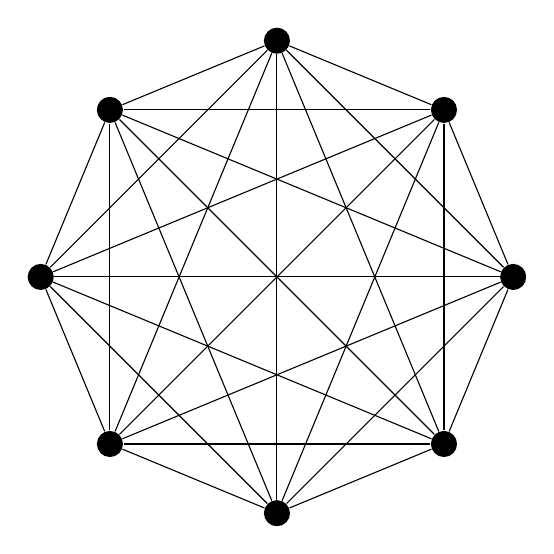
\begin{tikzpicture}
            \graph {subgraph K_n[nodes={circle,fill=black},empty nodes,n=8,clockwise,radius=30mm]};
        \end{tikzpicture}
        \caption{}
        \label{fig:a}
    \end{subfigure}
    \begin{subfigure}{0.45\textwidth}
        \centering            
        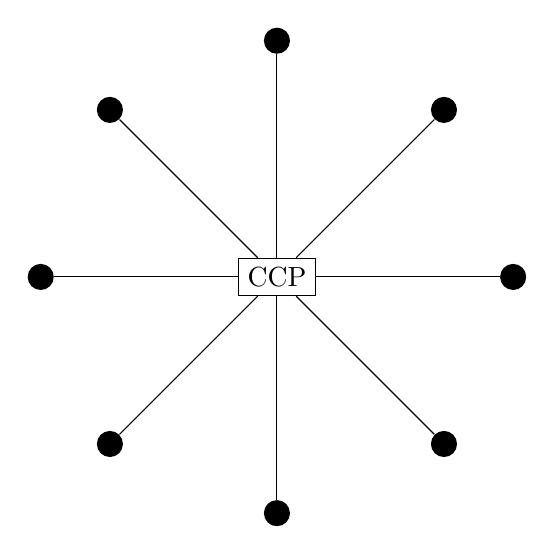
\begin{tikzpicture}
            \draw node[rectangle, draw] at (360:0mm) (centre) {CCP};
            \foreach \n in {1,...,8}{
                \draw node[circle,fill=black] at ({\n*45}:30mm) (n\n) {};
                \draw (centre) -- (n\n);
                }
        \end{tikzpicture}
        \caption{}
        \label{fig:b}
    \end{subfigure}
    \caption{}
	\label{fig:otc}
\end{figure}

\ref{fig:a} represents a series of bilateral agreements between 8 market participants. It is the traditional way OTC markets have operated. \ref{fig:b} shows how OTC markets would operate with a single central counterparty (CCP) acting as a clearing house.

\subsubsection*{Futures Trades vs. OTC Trades}

Regardless of how transactions are cleared, initial margin when provided in the form of cash usually earns interest. The daily variation margin provided by a clearing house member for futures contracts does not earn interest. This is because the variation margin constitutes the daily settlement. Transactions in the OTC market, whether cleared through CCPs or cleared bilaterally, are usually not settled daily. For this reason, the daily variation margin that is provided by the member of a CCP or, as a result of a CSA, earns interest when it is in the form of cash.

\subsection{Market Quotes}
\bigskip

\begin{definition*}
    We begin with a couple definitions.
    \begin{definition}[Opening price]\label{def:open}
        The price at which contracts trade at the start of the trading day.
    \end{definition}
    \begin{definition}[Settlement price]\label{def:settle}
        The \emph{settlement price} is the price used for calculating daily gains and losses and margin requirements. It is usually calculated as the price at which the contract traded at the end of the trading day.
    \end{definition}
    \begin{definition}[Change]\label{def:change}
        The difference between today's settlement price and yesterday's settlement price.
    \end{definition}
    \begin{definition}[Trading volume]\label{def:vol}
        The number of contracts traded in a day.
    \end{definition}
    \begin{definition}[Open interest]\label{def:open2}
        The number of outstanding contracts i.e. short/long positions.
    \end{definition}
    \begin{definition}[Normal market]\label{def:normal}
        A futures market where price \emph{increases} with maturity.
    \end{definition}
    \begin{definition}[Inverted market]\label{def:invert}
        A futures market where price \emph{decreases} with maturity.
    \end{definition}
\end{definition*} 

\subsubsection*{Delivery}

The seller (party with the short position) decides when to deliver. When the seller decides to deliver, the exchange must choose a party with a long position (a buyer) to accept delivery. This may very well be a different buyer than the one who initially entered the contract. The usual rule chosen by the exchange is to pass the notice of intention to deliver on to the party with the oldest outstanding long position. Parties with long positions must accept delivery notices. However, if the notices are transferable, traders with long positions have a short period of time to find another party with a long position that is prepared to take delivery in place of them.

\subsubsection*{Cash Settlement}

Some financial futures are settled in cash, as it is inconvenient or impossible to deliver the underlying asset.

\subsection{Types of Traders and Types of Orders}
\bigskip

\begin{definition*}
    There are two main types of traders executing trades: \emph{futures commission merchants} (FCMs) and \emph{locals}.
    \begin{definition}[Futures commission merchant]\label{def:merch}
        FCMs follow the instructions of their clients and charge a
        commission for their service.
    \end{definition}
    \begin{definition}[Locals]
        \emph{Locals} trade on their personal account.
    \end{definition}
\end{definition*}

Individuals, whether locals or clients of FCMs can be categorised as hedgers, speculators, or arbitrageurs as seen in \ref{ssec:types}.

\begin{definition*}
    There are three types of speculators.
    \begin{definition}[Scalpers]\label{def:scalp}
        \emph{Scalpers} are watching for very short-term trends (e.g. a couple of minutes) and attempt to profit from small changes in the contract price.
    \end{definition}
    \begin{definition}[Day traders]
        \emph{Day traders} hold their positions for less than one trading day. They are unwilling to take the risk that adverse news will occur overnight.
    \end{definition}
    \begin{definition}[Position traders]
        \emph{Position traders} hold their positions for much longer periods of time. They hope to make significant profits from major movements in the markets.
    \end{definition}
\end{definition*}

\subsubsection*{Orders}
\bigskip

\begin{definition*}
    There are quite a few types of orders.
    \begin{definition}[Market order]
        A \emph{market order} is a request that a trade be carried out immediately at the best price available in the market. The order is placed with a broker.
    \end{definition}
    \begin{definition}[Limit order]
        A \emph{limit order} specifies a price. That is, the order is only executed if the specified price or a more favourable one is reached.
    \end{definition}
    \begin{definition}[Stop-loss order]
        A \emph{stop-loss order} also specifies a price. The order is executed
        at the best available price once a bid or ask is made at that particular price or a less-favourable one.
    \end{definition}
    \begin{definition}[Market-if-touched (MIT) order]
        An \emph{MIT order} is executed at the best available price after a trade occurs at a specified price or one that is more favourable. This is also known as a \emph{board order}.
    \end{definition}
    \begin{definition}[Discretionary order]
        A \emph{discretionary order} is traded as a market order except that  execution may be delayed at the broker's discretion in an attempt to get a better price.
    \end{definition}
    \begin{definition}[Time-of-day order]
        A \emph{time-of-day order} specifies a particular period of time during the day when the order can be executed.
    \end{definition}
    \begin{definition}[Open order]
        An \emph{open order} is in effect until executed or until the end of trading in the particular contract. 
    \end{definition}
    \begin{definition}[Fill-or-kill order]
        A \emph{fill-or-kill order} must be executed immediately on receipt or not at all.
    \end{definition}
\end{definition*}

\subsubsection*{Regulation}

In the US futures markets are regulated by the CFTC which looks after public interest in a number of ways:

\begin{itemize}
    \item Ensures prices are communicated to the public and that futures traders report their outstanding positions if they are above certain levels
    \item Licenses all individuals who offer their services to the public in futures trading
    \item Deals with complaints and ensures disciplinary action is taken where appropriate complaints 
\end{itemize}

Another regulatory organisation is the NFA which combats fraud among other things.

\subsection{Accounting and tax}

\subsubsection*{Accounting}

Accounting standards require changes in the market value of a futures contract to be recognized when they occur unless the contract qualifies as a hedge. If the contract does qualify as a hedge, gains or losses are generally recognized for accounting purposes in the same period in which the gains or losses from the item being hedged are recognized. The latter treatment is referred to as hedge accounting.

\begin{eg}
    Consider a company with a December year-end. In September 2020 it buys a March 2021 corn futures contract and closes out the position at the end of February 2021. Suppose that the futures prices are 350 cents per bushel when the contract is entered into, 370 cents per bushel at the end of 2020, and 380 cents per bushel when the contract is closed out. The contract is for the delivery of 5000 bushels. If the contract does not qualify as a hedge, the gains for accounting purposes are \[5000 \times (3.70 - 3.50) = \$1000\] in 2020 and \[5000 \times (3.80 - 3.70) = \$500\] in 2021. If the company is hedging the purchase of 5000 bushels of corn in February 2021 so that the contract qualifies for hedge accounting, the entire gain of \$1500 is realized in 2021 for accounting purposes.
\end{eg}

\subsubsection*{Tax}

Two key issues are the nature of a taxable gain or loss and the timing of the recognition of the gain or loss. Gains or losses are either classified as capital gains or losses or alternatively as part of ordinary income.

\begin{itemize}
    \item For a corporate taxpayer, capital gains are taxed at the same rate as ordinary income, and the ability to deduct losses is restricted
    \item For a non-corporate taxpayer, short-term capital gains are taxed at the same rate as ordinary income, but long-term capital gains (gains from the sale of an asset held over a year) are subject to a maximum capital gains tax rate of 20\%
    \item Taxpayers earning income above certain thresholds pay an additional 3.8\% on all investment income
\end{itemize}

Tax regulations define a hedging transaction as a transaction entered into in the normal course of business primarily for one of the following reasons:

\begin{enumerate}
    \item To reduce the risk of price changes or currency fluctuations with respect to property that is held or to be held by the taxpayer for the purposes of producing ordinary income
    \item To reduce the risk of price or interest rate changes or currency fluctuations with respect to borrowings made by the taxpayer
\end{enumerate}

\subsection{Forward vs. Futures Contracts}

\begin{table}[h]
    \centering
    \begin{tabular}{|l|l|}
        \hline
        \emph{Forward} & \emph{Futures} \\\hline
        Traded OTC & Traded on an exchange \\
        Not standardised & Standardised \\
        Usually one specified delivery date & Range of delivery dates \\
        Settled at end of contract & Settled daily \\
        Delivery or final cash settlement usually takes place & Contract is usually closed out prior to maturity \\
        Some credit risk & Virtually no credit risk \\\hline
    \end{tabular}
    \caption{}
\end{table}